%% ID: launching_a_rocket
%% TITLE: Launching a Rocket
%% TYPE: question
%% QUESTIONTYPE: symbolic
%% CONCEPTS: momentum, newtonii, newtoniii
%% VIDEOS: 
%% LEVEL: 4
%% TOPIC: mechanics/dynamics
%% ORDER: 8

\begin{problem}[HE+_Rocket] %USED
{A rocket with initial mass \vari{M_{0}} and exhaust speed \vari{v} is sitting on its launch pad. Its engines eject mass at a constant rate of magnitude \valuedef{\lvert\frac{\d M}{\d t}\rvert}{\mu}{}.
\begin{enumerate}
	\item What is the initial acceleration, \vari{a_{0}}?
	\item Given that \valuedef{M_{0}}{1\times 10^{6}}{kg}, \valuedef{v}{2000}{m\,s\sup{-1}} and we require \valuedef{a_{0}}{0.5}{m\,s\sup{-2}}, what must \vari{\mu} be?
\end{enumerate}
}{
\stress{Adapted with permission from HE+.}
}{This question is a straightforward introduction to rocket questions.
\begin{enumerate}
	\item To find the initial acceleration, first consider the momentum change of the mass being ejected from the back of the rocket. Newton's Second Law gives us \vari{\vtr{F}}{\frac{\d p}{\d t}}{\vtr{v}\frac{\d M}{\d t}}{} since the exhaust velocity is a constant. This force acts on the mass being ejected to push it downwards, and so Newton's Third Law tells us there is an equal force pointing upwards acting on the rocket. So the thrust of the rocket is \vari{T} $=$ \valuedef{v\frac{\d M}{\d t}}{v\mu}{} upwards, but note that the \vari{\frac{\d M}{\d t}} here is the increase of mass outside the engine, not the decrease in mass of the spaceship. The two are of equal magnitude, \vari{\mu}, but opposite sign. Figure \ref{fig:Dynamics_rocket_force} illustrates the situation.

\begin{figure}[h]
	\centering
	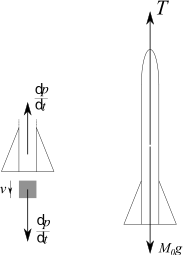
\includegraphics[width=0.3\textwidth]{../../../figures/Dynamics_rocket_force.eps}
	\caption{}\label{fig:Dynamics_rocket_force}
\end{figure}

It is then simply a case of finding the net force and applying Newton's Second Law again:
\begin{equation*} 
\text{Net Force} &= T - M_{0}g = M_{0}a_{0}
\end{equation*}
and so we find the acceleration:
\begin{eqnarray*} 
a_0 &= \frac{T - M_{0}g}{M_{0}} \\ 
&= \frac{\left(v\mu\right) - M_{0}g}{M_{0}} \\ 
&= \frac{\mu v}{M_{0}} - g 
\end{eqnarray*}
	\item Rearranging the expression to find \vari{\mu} gives:
\begin{eqnarray*} 
\mu &= \frac{(a_0 + g)M_{0}}{v} \\ 
&= \frac{(0.5 + 9.8)(1 \times 10^{6})}{2000} \\ 
&= \mbox{\quantity{5150}{kg\,s\sup{-1}}} 
\end{eqnarray*}
\end{enumerate}	
}
\end{problem}